\documentclass[10pt, xcolor=table]{beamer}

\setbeamertemplate{note page}[default]
%\setbeameroption{hide notes}
\setbeameroption{show notes}
\setbeamerfont{footnote}{size=\tiny}

\usetheme[progressbar=frametitle]{metropolis}
\usepackage{appendixnumberbeamer}

\usepackage{booktabs}
\usepackage[scale=2]{ccicons}

\usepackage{pgfplots}
\usepgfplotslibrary{dateplot}
\usepackage{multicol}
\setlength{\columnsep}{1.5cm}
\usepackage{multirow}


\usepackage{animate}
\usepackage{lmodern}
\usepackage[T1]{fontenc}
\usepackage{mathtools}
\usepackage{graphicx}
\usepackage{caption}
\usepackage{tikz}
\usepackage{stackengine}
\usepackage{array}
\usetikzlibrary{positioning}
\usepackage{tabulary}

\usepackage[math]{cellspace}
\cellspacetoplimit 2pt
\cellspacebottomlimit 2pt


\definecolor{set1}{RGB}{228, 26, 28}
\definecolor{set2}{RGB}{77, 175, 74}
\definecolor{set3}{RGB}{255, 127, 0}
\definecolor{set4}{RGB}{166, 86, 40}
\definecolor{set5}{RGB}{153, 153, 153}

\usepackage{xspace}
\newcommand{\themename}{\textbf{\textsc{metropolis}}\xspace}

\newcommand\Fontvi{\fontsize{8}{9}\selectfont}
\newcommand\Fontvr{\fontsize{6}{7}\selectfont}

\setbeamerfont{parent A}{size=\small}

\DeclarePairedDelimiter\abs{\lvert}{\rvert}%
\DeclarePairedDelimiter\norm{\lVert}{\rVert}%
\makeatletter
\let\oldabs\abs
\def\abs{\@ifstar{\oldabs}{\oldabs*}}
\let\oldnorm\norm
\def\norm{\@ifstar{\oldnorm}{\oldnorm*}}
\makeatother
\newcommand*{\Value}{\frac{1}{2}x^2}%

\title{Digital Transformation of Healthcare}
\subtitle{Evaluating Predictions \& Data Quality}
% \date{\today}
\date{}
\author{Michoel Snow, MD PhD, Glen Ferguson, PhD}
\institute{Center for Health Data Innovations}
% \titlegraphic{\hfill\includegraphics[height=1.5cm]{logo.pdf}}

\begin{document}

\maketitle


\begin{frame}{Objectives}
	After this lecture students will be able to 
	\begin{itemize}
		\item Calculate common classification and regression metrics
		\item Describe the role of simple classification metrics
		\item Evaluate the implementation of metrics for a study 
		\item Articulate the information underlying common compound classification metrics 
		\item Classify regression metrics 
		\item Connect regression metric outcomes to facets of the associated models
		\item Identify transition points which can affect data quality
		\item Discuss methods for measuring and evaluating data quality 
	\end{itemize}%
\end{frame}


\begin{frame}
	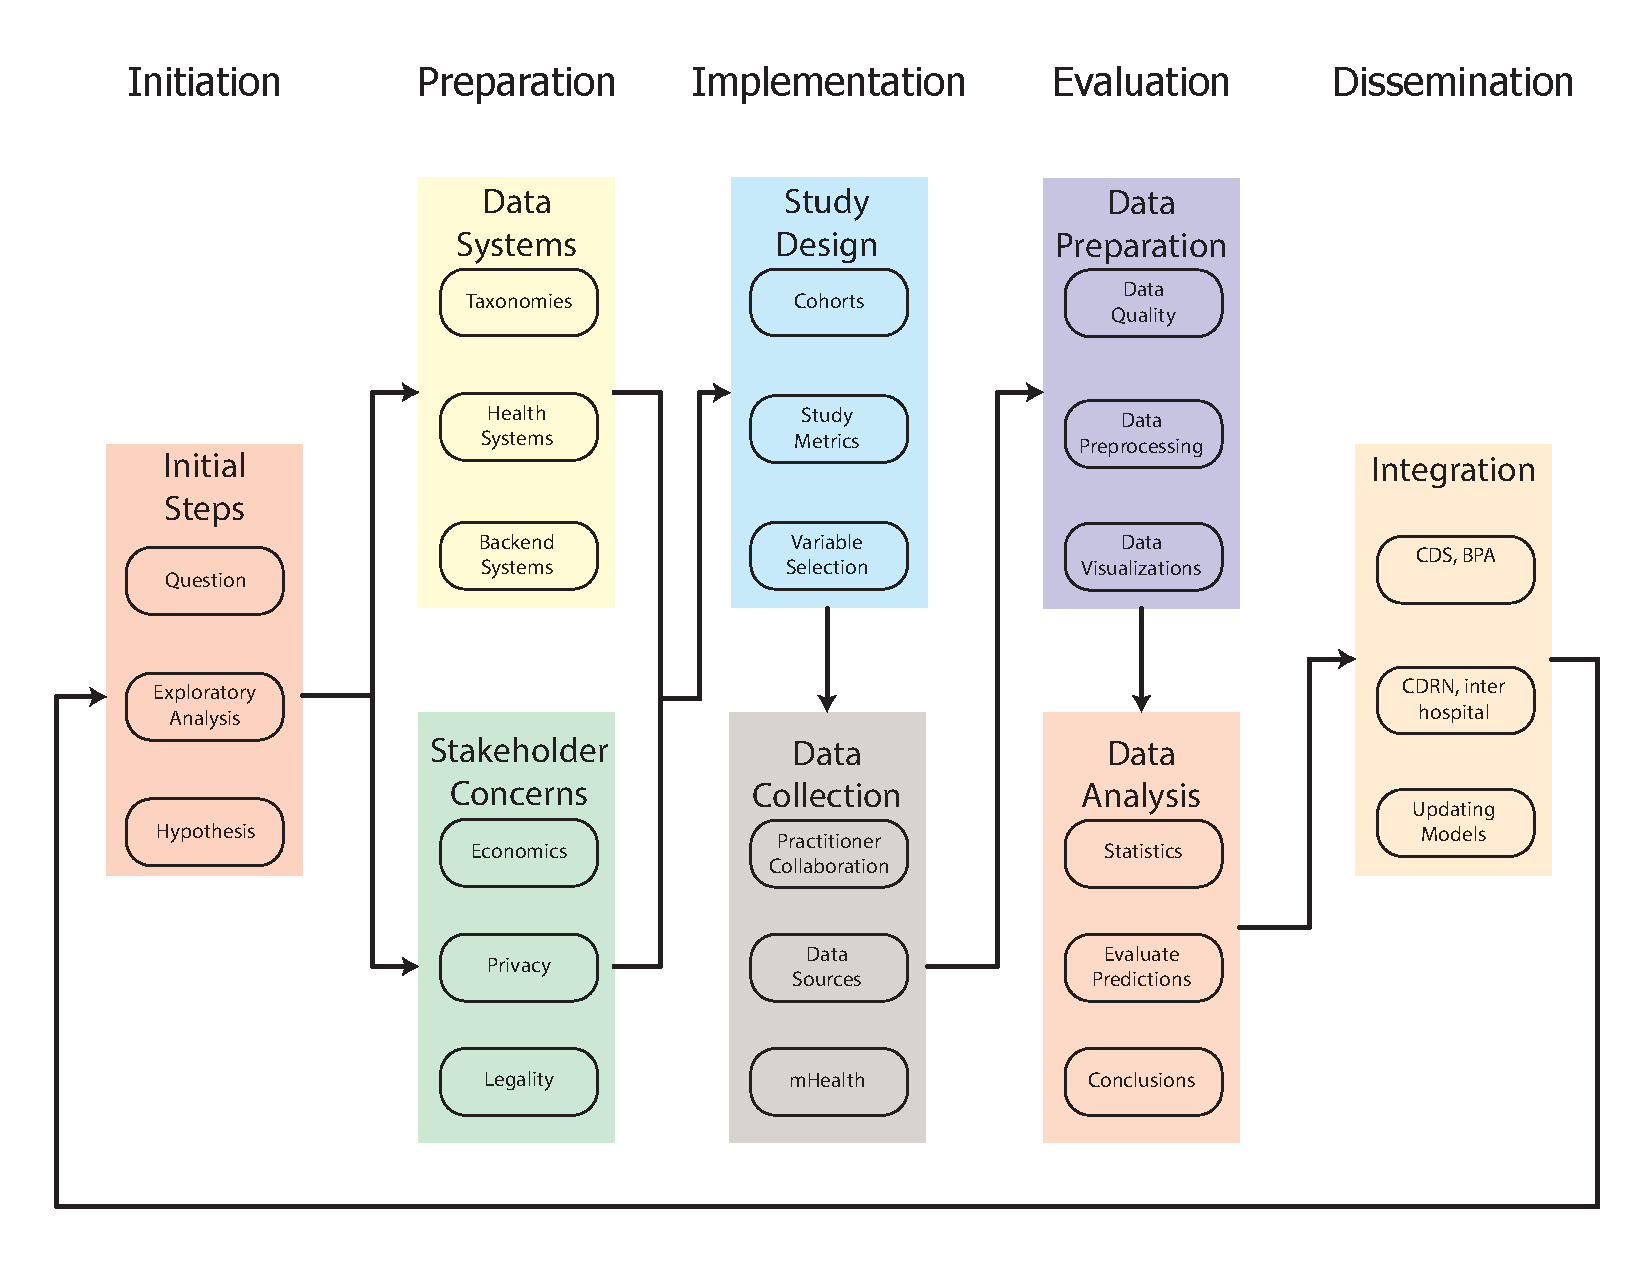
\includegraphics[height=\textheight]{../../informatics_pipeline.pdf}
\end{frame}

\section{Metrics for Evaluation of Classification Models}

\begin{frame}{Clinical Cases}
	\begin{table}
		\begin{tabular}{| p{2cm} | c | p{2cm} | c | c | c | c |}
			\hline
			Case & Prevalence & Criteria & TP & FP & TN & FN  \\ \hline
			LDCT for lung cancer & UN & non-calcified nodule $\geq 4mm$ & 649 & 17497 & 55324 & UN \\ \hline
		\end{tabular}
	\end{table}
\end{frame}

\begin{frame}{Clinical Cases}
	\begin{table}
		\begin{tabulary}{1\textwidth}{| L | C | C | L | L | C | C |}
			\hline
			Case & Prevalence & Criteria & TP & FP & TN & FN  \\ \hline
			LDCT for lung cancer & UN & non-calcified nodule $\geq 4mm$ & 649 & 17497 & 55324 & UN \\ \hline
		\end{tabulary}
	\end{table}
\end{frame}


% National Lung Screening Trial Research Team, Aberle DR, Adams AM, Berg CD,
%Black WC, Clapp JD, Fagerstrom RM, Gareen IF, Gatsonis C, Marcus PM, Sicks JD.
%Reduced lung-cancer mortality with low-dose computed tomographic screening. N
%Engl J Med. 2011 Aug 4;365(5):395-409. doi: 10.1056/NEJMoa1102873. Epub 2011 Jun 
%29. PubMed PMID: 21714641; PubMed Central PMCID: PMC4356534.


\begin{frame}{Confusion Matrix}
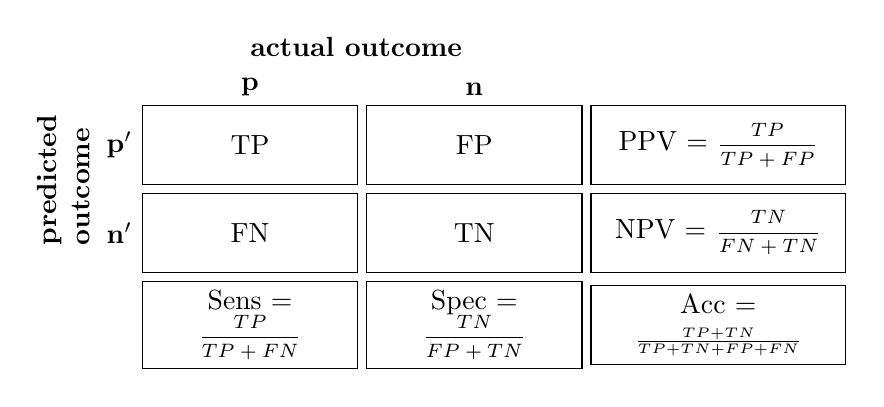
\begin{tikzpicture}[ampersand replacement=\&,
box/.style={draw,rectangle,minimum size=1cm,text width=2.5cm,align=center},
box2/.style={draw,rectangle,minimum size=1cm,text width=3cm,align=center}]
\matrix (conmat) [row sep=.1cm,column sep=.1cm] {
\node (tpos) [box,
    label=left:\( \mathbf{p'} \),
    label=above:\( \mathbf{p} \),
    ] {TP};
\&
\node (fpos) [box,
    label=above:\textbf{n}] {FP};
\&
\node (ppv) [box2] {PPV = \scriptsize{$\dfrac{TP}{TP+FP}$}};
\\
\node (fneg) [box,
    label=left:\( \mathbf{n'} \)] {FN};
\&
\node (tneg) [box] {TN};
\&
\node (npv) [box2] {NPV = \scriptsize{$\dfrac{TN}{FN+TN}$}};
\\
\node (sens) [box] {Sens = \scriptsize{$\dfrac{TP}{TP+FN}$}};
\&
\node (spec) [box] {Spec = \scriptsize{$\dfrac{TN}{FP+TN}$}};
\&
\node (acc) [box2] {Acc = \scriptsize{$\frac{TP+TN}{TP+TN+FP+FN}$}};
%\node (f1) [box2] {F1 = \scriptsize{$\dfrac{2 \times Sens \times PPV}{PPV + Sens}$}};
\\
};
\node [rotate=90, anchor=center,xshift=.35cm, left=1cm of tpos, text width=1.5cm,align=center ] {\textbf{predicted \\ outcome}};
\node [above=0.5cm of fpos,xshift=-1.5cm,align=left] {\textbf{actual outcome}};
\end{tikzpicture}
\end{frame}

%F1 &= \frac{2 \times Sens \times PPV}{Sens + PPV} \\

\begin{frame}{Confusion Matrix}
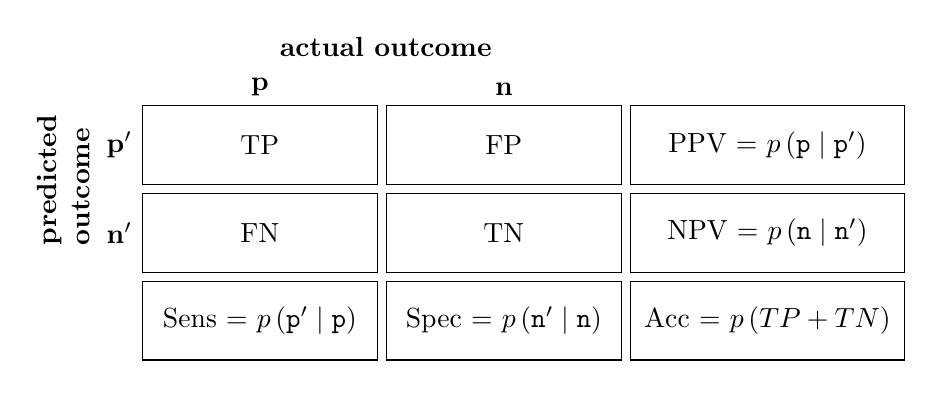
\begin{tikzpicture}[ampersand replacement=\&,
box/.style={draw,rectangle,minimum size=1cm,text width=2.75cm,align=center},
box2/.style={draw,rectangle,minimum size=1cm,text width=3.25cm,align=center}]
\matrix (conmat) [row sep=.1cm,column sep=.1cm] {
\node (tpos) [box,
    label=left:\( \mathbf{p'} \),
    label=above:\( \mathbf{p} \),
    ] {TP};
\&
\node (fpos) [box,
    label=above:\textbf{n}] {FP};
\&
\node (ppv) [box2] {PPV = {$p\left(\texttt{\textbf{p}}\mid \texttt{\textbf{p}}'\right)$}};
\\
\node (fneg) [box,
    label=left:\( \mathbf{n'} \)] {FN};
\&
\node (tneg) [box] {TN};
\&
\node (npv) [box2] {NPV = {$p\left(\texttt{\textbf{n}}\mid \texttt{\textbf{n}}'\right)$}};
\\
\node (sens) [box] {Sens = {$p\left(\texttt{\textbf{p}}'\mid \texttt{\textbf{p}}\right)$}};
\&
\node (spec) [box] {Spec = {$p\left(\texttt{\textbf{n}}'\mid \texttt{\textbf{n}}\right)$}};
\&
\node (acc) [box2] {Acc = {$p\left(TP + TN\right)$}};
\\
};
\node [rotate=90, anchor=center,xshift=.35cm, left=1cm of tpos, text width=1.5cm,align=center ] {\textbf{predicted \\ outcome}};
\node [above=0.5cm of fpos,xshift=-1.5cm,align=left] {\textbf{actual outcome}};
\end{tikzpicture}

\end{frame}




%\begin{frame}{Confusion Matrix}
%\vspace{4em}
%\begin{center}
%\begin{tikzpicture}[transform canvas={scale=0.75}, ampersand replacement=\&,
%box/.style={draw,rectangle,minimum size=1cm,text width=2.75cm,align=center},
%box2/.style={draw,rectangle,minimum size=1cm,text width=3.25cm,align=center}]
%\matrix (conmat) [row sep=.1cm,column sep=.1cm] {
%\node (tpos) [box,
%    label=left:\( \mathbf{p'} \),
%    label=above:\( \mathbf{p} \),
%    ] {TP};
%\&
%\node (fpos) [box,
%    label=above:\textbf{n}] {FP};
%\&
%\node (ppv) [box2] {PPV = {$p\left(\texttt{\textbf{p}}\mid \texttt{\textbf{p}}'\right)$}};
%\\
%\node (fneg) [box,
%    label=left:\( \mathbf{n'} \)] {FN};
%\&
%\node (tneg) [box] {TN};
%\&
%\node (npv) [box2] {NPV = {$p\left(\texttt{\textbf{n}}\mid \texttt{\textbf{n}}'\right)$}};
%\\
%\node (sens) [box] {Sens = {$p\left(\texttt{\textbf{p}}'\mid \texttt{\textbf{p}}\right)$}};
%\&
%\node (spec) [box] {Spec = {$p\left(\texttt{\textbf{n}}'\mid \texttt{\textbf{n}}\right)$}};
%\&
%\node (acc) [box2] {Acc = {$p\left(TP + TN\right)$}};
%%\node (f1) [box2] {F1 = \scriptsize{$\dfrac{2 \times Sens \times PPV}{PPV + Sens}$}};
%\\
%};
%\node [rotate=90, anchor=center,xshift=.35cm, left=1cm of tpos, text width=1.5cm,align=center ] {\textbf{predicted \\ outcome}};
%\node [above=0.5cm of fpos,xshift=-1.5cm,align=left] {\textbf{actual outcome}};
%\end{tikzpicture}
%\end{center}
%\vspace{3em}
%
%\begin{table}
%	\scriptsize
%	\begin{tabular}{c c c}
%		Parameter & Interpretation & Inappropriate for \\ \hline \hline
%		Accuracy & Overall proximity of test to reality & Imbalanced sample sizes \\	
%		Sensitivity  &  & \\ 
%		Specificity  &  & \\
%		PPV  &  &  \\
%		NPV &  &  \\
%	\end{tabular}
%\end{table}
%\end{frame}













\begin{frame}{Confusion Matrix}
\vspace{4em}
\begin{center}
\begin{tikzpicture}[transform canvas={scale=0.75}, ampersand replacement=\&,
box/.style={draw,rectangle,minimum size=1cm,text width=2.75cm,align=center},
box2/.style={draw,rectangle,minimum size=1cm,text width=3.25cm,align=center}]
\matrix (conmat) [row sep=.1cm,column sep=.1cm] {
\node (tpos) [box,
    label=left:\( \mathbf{p'} \),
    label=above:\( \mathbf{p} \),
    ] {TP};
\&
\node (fpos) [box,
    label=above:\textbf{n}] {FP};
\&
\node (ppv) [box2] {PPV = {$p\left(\texttt{\textbf{p}}\mid \texttt{\textbf{p}}'\right)$}};
\\
\node (fneg) [box,
    label=left:\( \mathbf{n'} \)] {FN};
\&
\node (tneg) [box] {TN};
\&
\node (npv) [box2] {NPV = {$p\left(\texttt{\textbf{n}}\mid \texttt{\textbf{n}}'\right)$}};
\\
\node (sens) [box] {Sens = {$p\left(\texttt{\textbf{p}}'\mid \texttt{\textbf{p}}\right)$}};
\&
\node (spec) [box] {Spec = {$p\left(\texttt{\textbf{n}}'\mid \texttt{\textbf{n}}\right)$}};
\&
\node (acc) [box2] {Acc = {$p\left(TP + TN\right)$}};
%\node (f1) [box2] {F1 = \scriptsize{$\dfrac{2 \times Sens \times PPV}{PPV + Sens}$}};
\\
};
\node [rotate=90, anchor=center,xshift=.35cm, left=1cm of tpos, text width=1.5cm,align=center ] {\textbf{predicted \\ outcome}};
\node [above=0.5cm of fpos,xshift=-1.5cm,align=left] {\textbf{actual outcome}};
\end{tikzpicture}
\end{center}
\vspace{3em}

\begin{table}
	\scriptsize
	\begin{tabular}{c c c}
		Parameter & Interpretation & Inappropriate for \\ \hline \hline
		Accuracy &  Overall proximity of test to reality & Imbalanced sample sizes \\
		Sensitivity  & \onslide<2>{Chance of a false negative} &  \onslide<2>{Expensive testing/Mild disease}\\ 
		Specificity  &  \onslide<2>{Chance of a false positive} &  \onslide<2>{Cheap testing/Severe disease}\\
		PPV  & \onslide<2>{Sensitivity diagnostic utility} & \onslide<2>{Very high prevalence} \\
		NPV & \onslide<2>{Specificity diagnostic utility} & \onslide<2>{Very low prevalence} \\
	\end{tabular}
\end{table}
\end{frame}



%
%\begin{frame}{Confusion Matrix}
%\vspace{4em}
%\begin{center}
%\begin{tikzpicture}[transform canvas={scale=0.75}, ampersand replacement=\&,
%box/.style={draw,rectangle,minimum size=1cm,text width=2.75cm,align=center},
%box2/.style={draw,rectangle,minimum size=1cm,text width=3cm,align=center}]
%\matrix (conmat) [row sep=.1cm,column sep=.1cm] {
%\node (tpos) [box,
%    label=left:\( \mathbf{p'} \),
%    label=above:\( \mathbf{p} \),
%    ] {TP};
%\&
%\node (fpos) [box,
%    label=above:\textbf{n}] {FP};
%\&
%\node (ppv) [box2] {PPV = {$p\left(\texttt{\textbf{p}}\mid \texttt{\textbf{p}}'\right)$}};
%\\
%\node (fneg) [box,
%    label=left:\( \mathbf{n'} \)] {FN};
%\&
%\node (tneg) [box] {TN};
%\&
%\node (npv) [box2] {NPV = {$p\left(\texttt{\textbf{n}}\mid \texttt{\textbf{n}}'\right)$}};
%\\
%\node (sens) [box] {Sens = {$p\left(\texttt{\textbf{p}}'\mid \texttt{\textbf{p}}\right)$}};
%\&
%\node (spec) [box] {Spec = {$p\left(\texttt{\textbf{n}}'\mid \texttt{\textbf{n}}\right)$}};
%\&
%\node (acc) [box2] {Acc = {$p\left(TP + TN\right)$}};
%%\node (f1) [box2] {F1 = \scriptsize{$\dfrac{2 \times Sens \times PPV}{PPV + Sens}$}};
%\\
%};
%\node [rotate=90, anchor=center,xshift=.35cm, left=1cm of tpos, text width=1.5cm,align=center ] {\textbf{predicted \\ outcome}};
%\node [above=0.5cm of fpos,xshift=-1.5cm,align=left] {\textbf{actual outcome}};
%\end{tikzpicture}
%\end{center}
%\vspace{3em}
%
%\begin{table}
%	\scriptsize
%	\begin{tabular}{c c c}
%	Condition & Stats & Example \\ \hline \hline
%	High Sensitivity, Low Specificity & \textbf{p}$'$ $>>$ \textbf{n}$'$ & test is always  positive \\	
%	Low Sensitivity, High Specificity  & \textbf{n}$'$ $>>$ \textbf{p}$'$ & test is always negative \\
%	High PPV, Low NPV & \textbf{p} $>>$ \textbf{n} & high disease prevalence \\
%	Low PPV, High NPV & \textbf{n} $>>$ \textbf{p} & low disease prevalence \\
%	High PPV, Low Sensitivity & FN $>>$ FP & say they are negative most of the time for a high prevalence disease \\
%	High Sensitivity, Low NPV & & \\
%	High Specificity, Low NPV & & \\
%	High PPV, Low Specificity & & \\
%	\end{tabular}
%\end{table}
%
%\end{tabular}
%\end{frame}

\begin{frame}{Combined Statistics}

\begin{table}
	\scriptsize
	\begin{tabular}{c c c}
		Function of & Metric & Formula\\ \hline \hline \\ 
		Sensitivity, Specificity  & Positive Likelihood Ratio/ROC & $\dfrac{sensitivity}{1-specificity}$ \\ [1.5em]
		Sensitivity, Specificity  & Negative Likelihood Ratio & $\dfrac{1-sensitivity}{specificity}$ \\ [1.5em]
		Sensitivity, PPV & F1 score & $\dfrac{2}{\dfrac{1}{sensitivity} + \dfrac{1}{PPV} }$  \\ [4em]
		TP, TN, FP, FN & Matthews correlation coefficient & \tiny{$\dfrac{TP\times TN-FP\times FN}{\sqrt{\left(TP + FP\right)\left(TP+FN\right)\left(TN+FP\right)\left(TN+FN\right)}}$} \\
	\end{tabular}
\end{table}
\end{frame}


\begin{frame}{Likelihood Ratios}
	\begin{center}
		Does a test result change the probability that a person has a certain condition?
	\end{center}
	\begin{align*}
		LR+ &= \dfrac{sensitivity}{1 - specificity} = \dfrac{P\left(T+ \mid D+\right)}{P\left(T+ \mid D-\right)} \\[1.5em]
		LR- &= \dfrac{1 - sensitivity}{specificity} = \dfrac{P\left(T- \mid D+\right)}{P\left(T- \mid D-\right)}
	\end{align*}
%	\begin{center}
%		
%	\end{center}
\end{frame}

\begin{frame}{Likelihood Ratios}
	\begin{center}
		\rowcolors{2}{gray!25}{white}
		\begin{tabular}{c c}
			\rowcolor{gray!50}
			Likelihood Ratio & Approximate Change in Probability(\%) \\ \hline
			0.1 & -45 \\
			0.2 & -30 \\
			0.5 & -15 \\
			1 & 0 \\
			2 & +15 \\
			5 & +30 \\
			10 & +45
		\end{tabular} \\[2em]
		Change in post test probability $\approx 0.2 \times \ln{LR}$ \footnote{{McGee, Steven. "Simplifying likelihood ratios." Journal of general internal medicine 17.8 (2002): 647-650.
APA	
}}
	\end{center}
\end{frame}


\begin{frame}{Hypothesis Testing}
	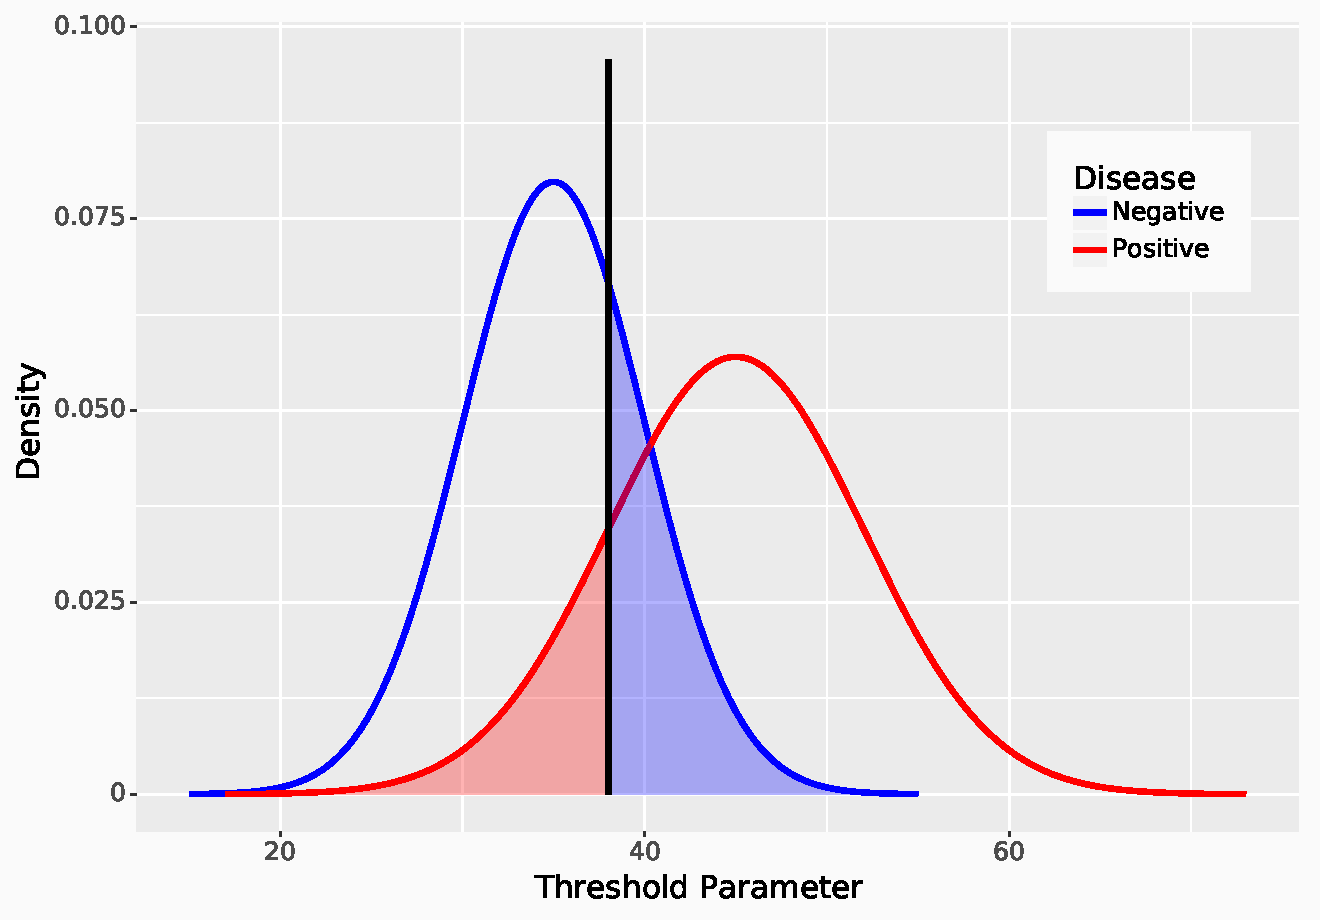
\includegraphics[height=0.8\textheight]{images/overlap_distr.pdf}
\end{frame}


\begin{frame}{Discrimination Thresholds}
	\begin{center}
		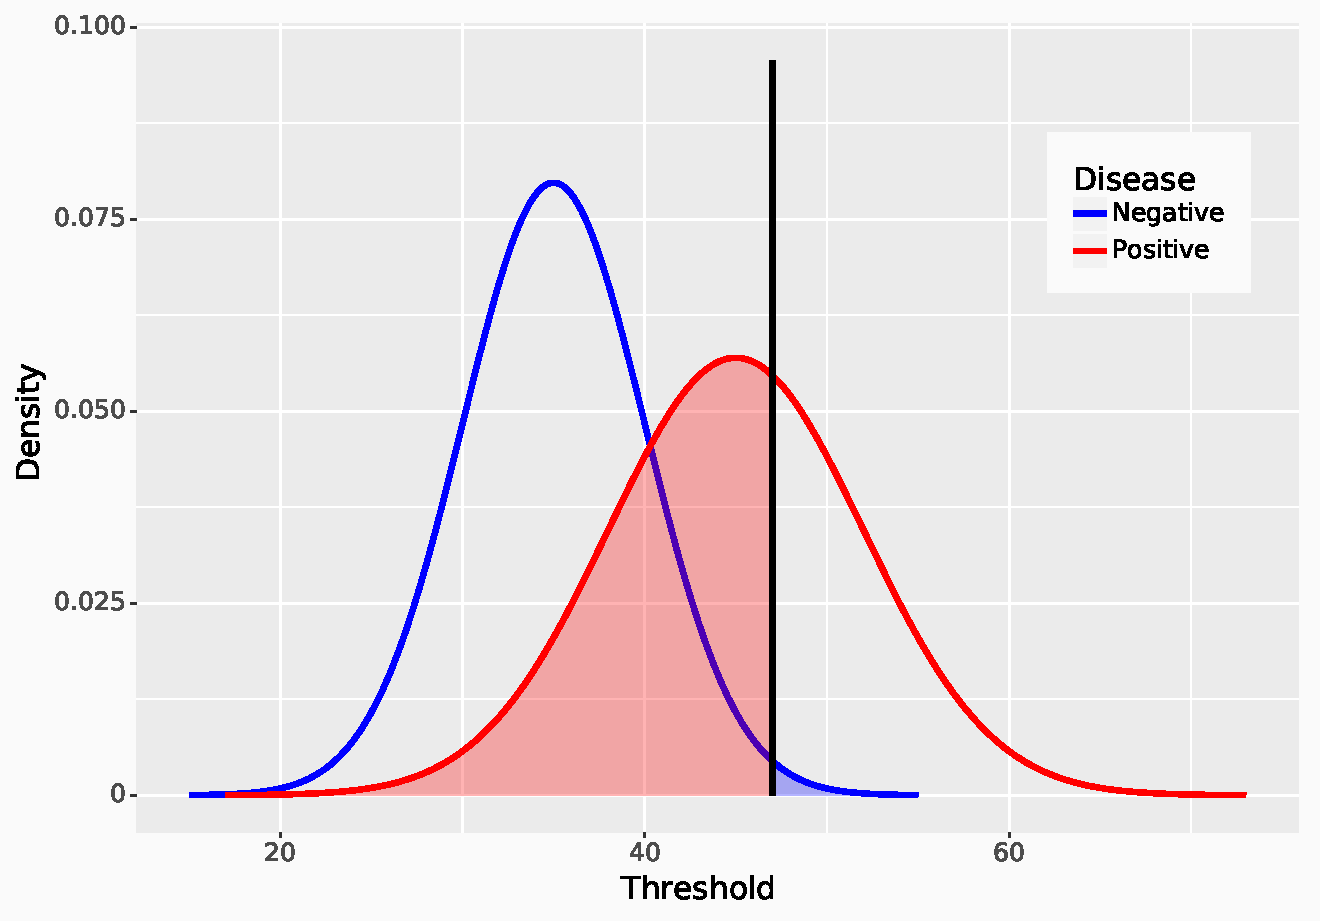
\includegraphics[height=0.45\textheight]{images/overlap_distr_thi.pdf}\\
		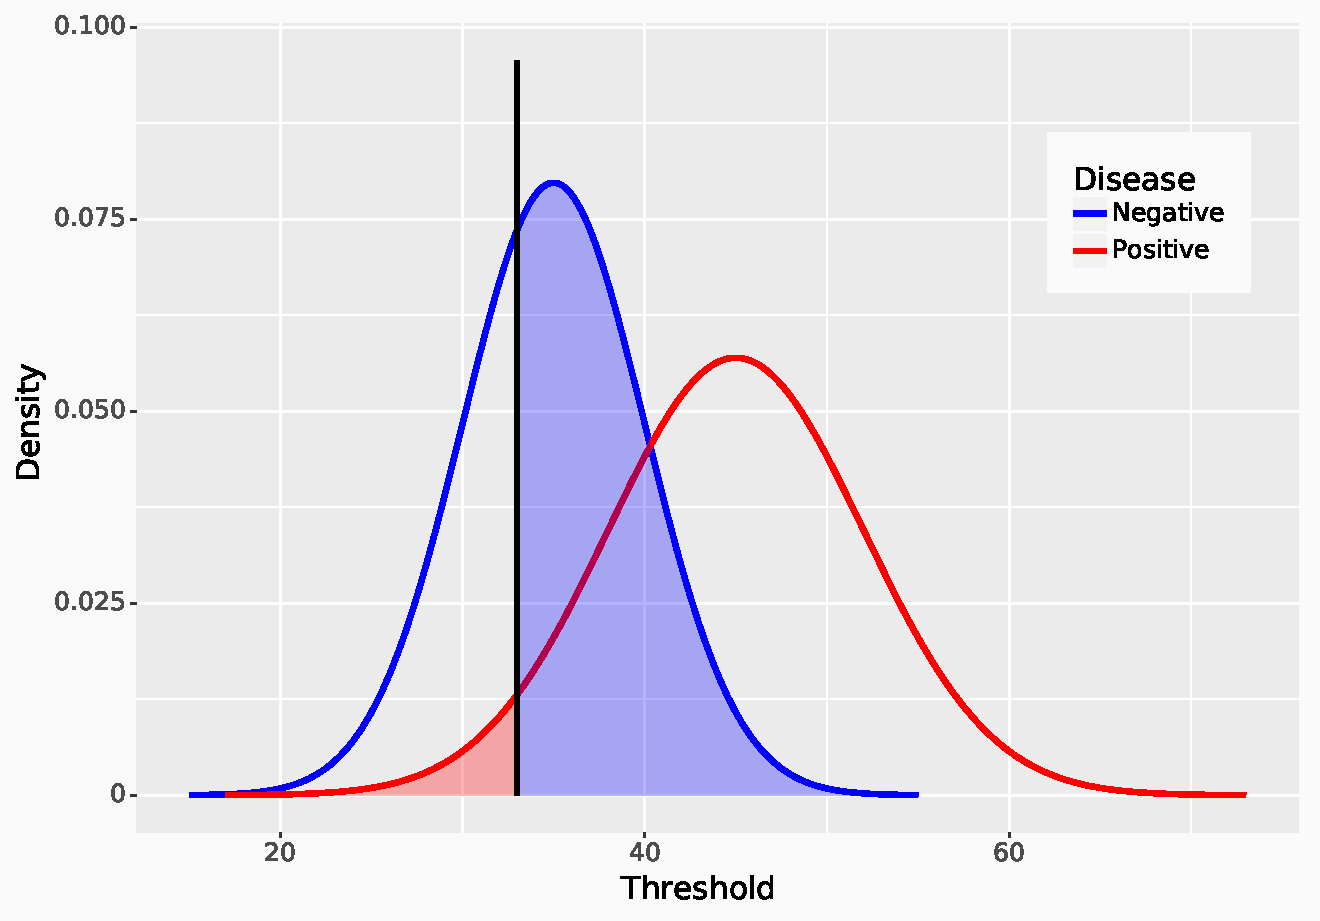
\includegraphics[height=0.45\textheight]{images/overlap_distr_tlow.pdf}
	\end{center}
\end{frame}

%\begin{frame}{Receiver Operating Characteristic}
%	\begin{center}
%		 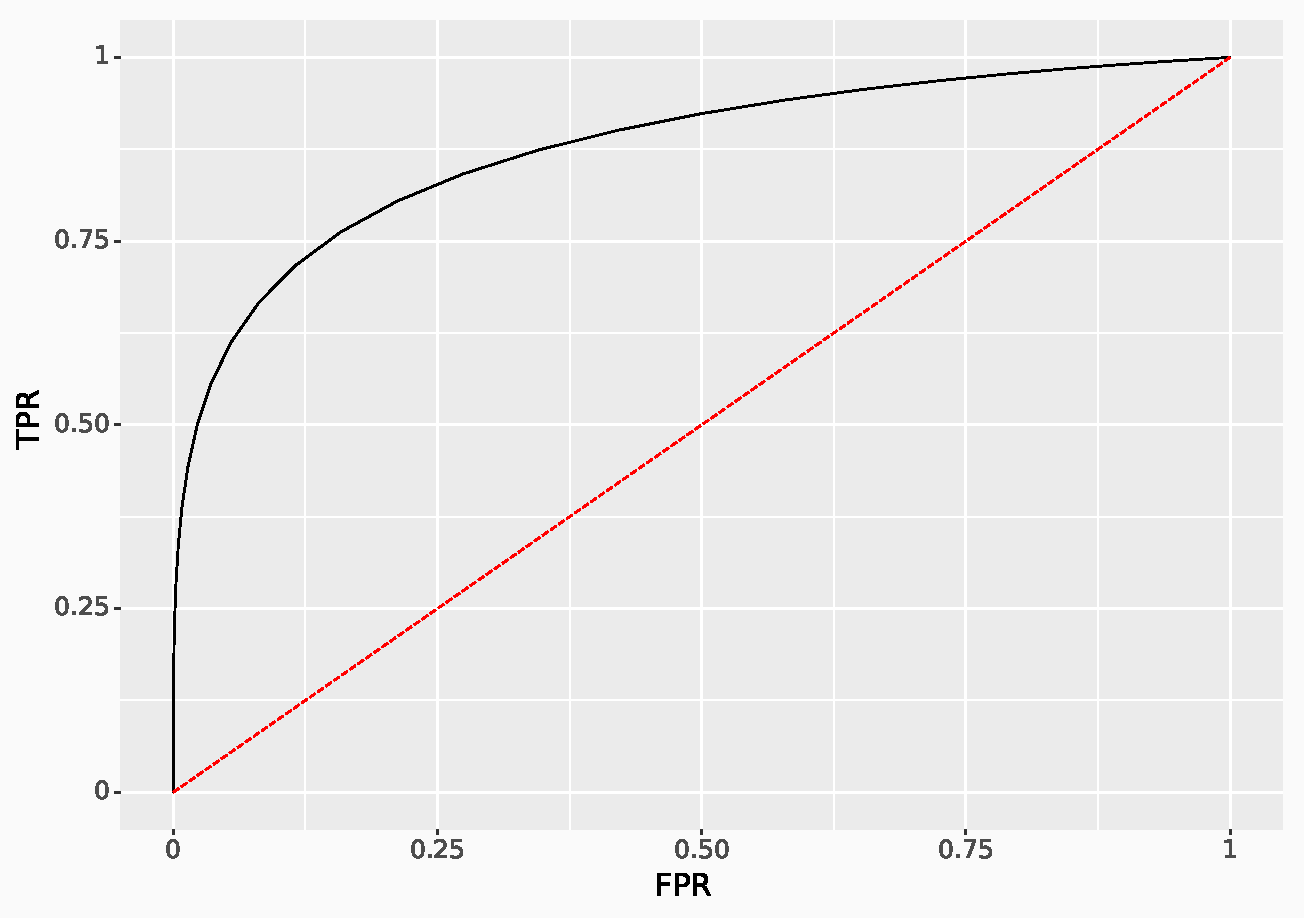
\includegraphics[height=0.8\textheight]{images/ROC.pdf}\\
%	\end{center}
%\end{frame}

\begin{frame}{Receiver Operating Characteristic}
	\begin{center}
		 \stackinset{r}{1em}{b}{3em}{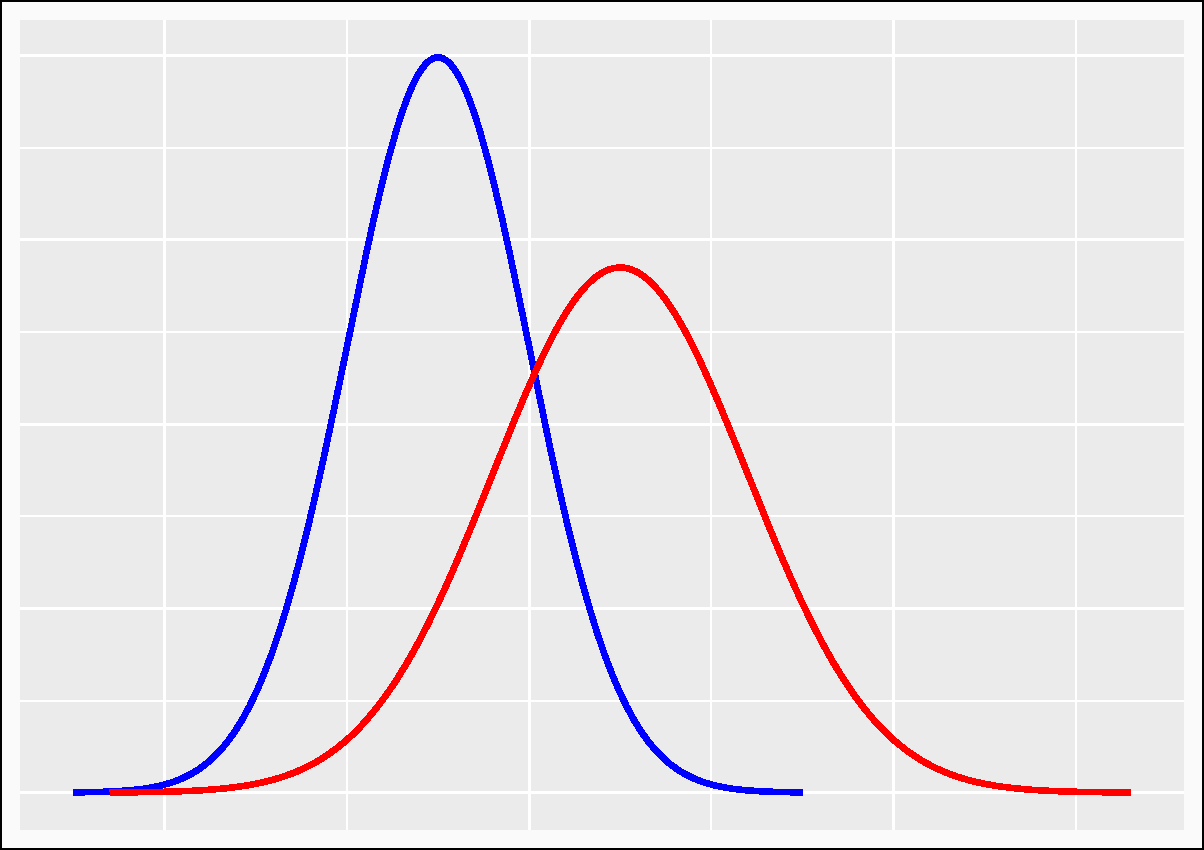
\includegraphics[width=1in]{images/overlap_distr_no_thresh.pdf}}
  {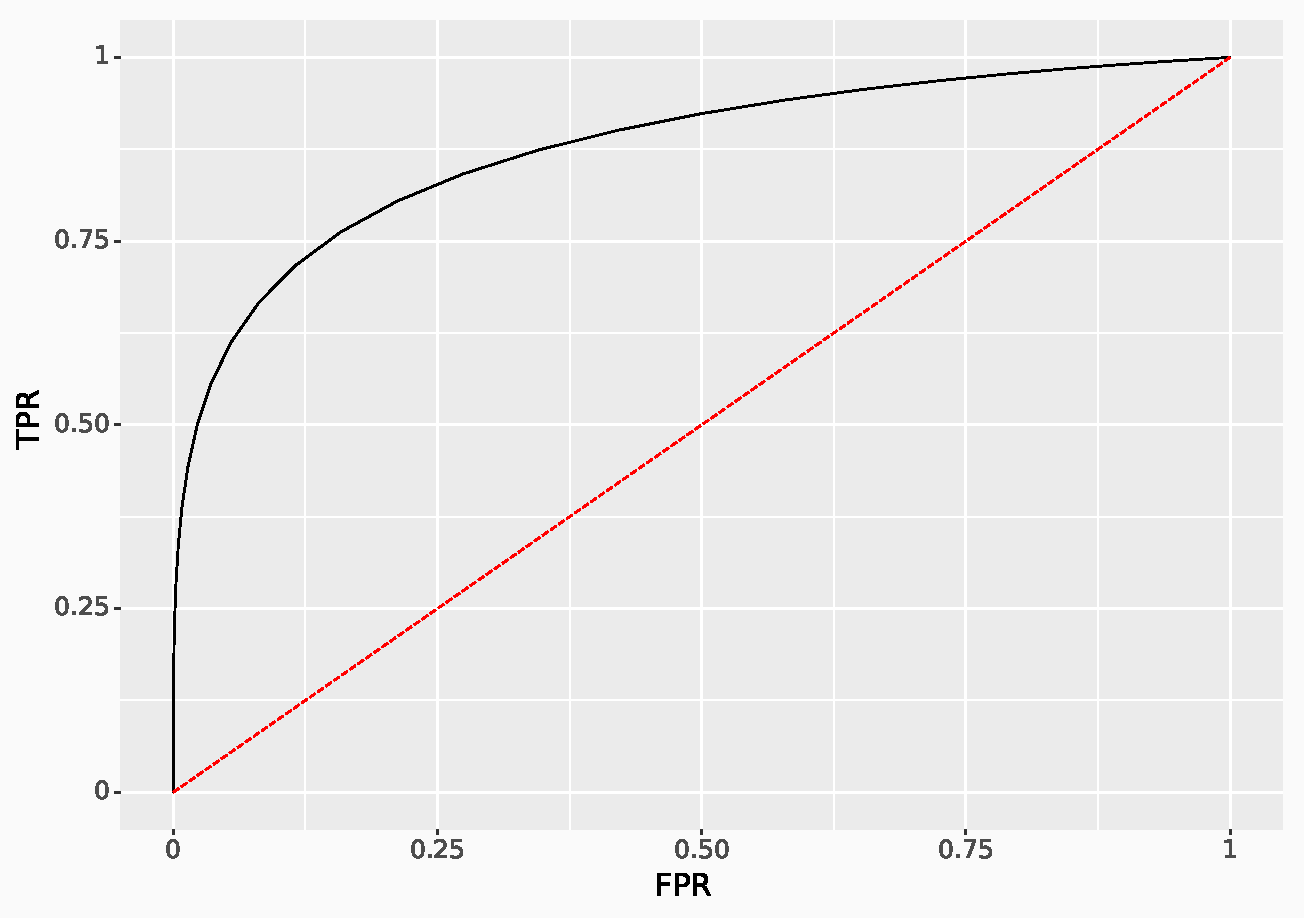
\includegraphics[width=0.9\textwidth]{images/ROC.pdf}}\\
  \onslide<2>{What does the Area Under the Curve (AUC) correspond to?} \\
  \onslide<2>{What does the diagonal correspond to?}
	\end{center}

	\note[item]<2>{Given a positive test result what are the chances that the subject is truly positive irrespective of prevalence?}	
	\note[item]<2>{PPV is threshold dependent, while AUC is threshold independent but variable dependent}	
\end{frame}

\begin{frame}{F1 Score}
\vspace{3em}
\begin{center}
\begin{tikzpicture}[transform canvas={scale=0.75}, ampersand replacement=\&,
box/.style={draw,rectangle,minimum size=1cm,text width=2.75cm,align=center},
box2/.style={draw,rectangle,minimum size=1cm,text width=3.25cm,align=center}]
\matrix (conmat) [row sep=.1cm,column sep=.1cm] {
\node (tpos) [box,
    label=left:\( \mathbf{p'} \),
    label=above:\( \mathbf{p} \),
    ] {TP};
\&
\node (fpos) [box,
    label=above:\textbf{n}] {FP};
\&
\node (ppv) [box2] {PPV = {$p\left(\texttt{\textbf{p}}\mid \texttt{\textbf{p}}'\right)$}};
\\
\node (fneg) [box,
    label=left:\( \mathbf{n'} \)] {FN};
\&
\node (tneg) [box] {TN};
\&
\node (npv) [box2] {NPV = {$p\left(\texttt{\textbf{n}}\mid \texttt{\textbf{n}}'\right)$}};
\\
\node (sens) [box] {Sens = {$p\left(\texttt{\textbf{p}}'\mid \texttt{\textbf{p}}\right)$}};
\&
\node (spec) [box] {Spec = {$p\left(\texttt{\textbf{n}}'\mid \texttt{\textbf{n}}\right)$}};
\&
\node (acc) [box2] {Acc = {$p\left(TP + TN\right)$}};
%\node (f1) [box2] {F1 = \scriptsize{$\dfrac{2 \times Sens \times PPV}{PPV + Sens}$}};
\\
};
\node [rotate=90, anchor=center,xshift=.35cm, left=1cm of tpos, text width=1.5cm,align=center ] {\textbf{predicted \\ outcome}};
\node [above=0.5cm of fpos,xshift=-1.5cm,align=left] {\textbf{actual outcome}};
\end{tikzpicture}
\end{center}
\vspace{1em}
	\begin{center}
		\begin{align*}
			F1 &= \dfrac{2}{\dfrac{1}{sensitivity} + \dfrac{1}{PPV} } = 2 \times \dfrac{PPV \cdot sensitivity}{PPV + sensitivity}
		\end{align*}\\[1em]
		How does F1 differ from AUC?
	\end{center}

\note[item]{F1 is sensitivity modified by prevalence.  So a low prevalence will hurt your F1 score but might not affect your AUC.  F1 is threshold specific and corresponds to a point on the ROC curve}	
	\note[item]{}	
	
\end{frame}



%\begin{frame}
%	\begin{itemize}
%		\item Sensitivity = TP:FN (say everyone is positive)
%		\item Specificity = TN:FP (say everyone is negative)
%		\item PPV = TP:FP (high prevalence disease)
%		\item NPV = TN:FN (low prevalence disease)
%		\item Accuracy = (TP $+$ TN):(FP $+$ FN)
%	\end{itemize}
%
%\end{frame}


%F1 &= \frac{2 \times Sens \times PPV}{Sens + PPV} \\



\section{Metrics for Evaluation of Regression Models}

\begin{frame}{Regression Metrics}
	\begin{itemize}
		\item What aspects of a model's predictions should I care about?
		\item What aspects of the model's predictions can I evaluate? 
	\end{itemize}

	\note[item]{
		\begin{itemize}
			\item Accuracy (bias), precision (variance)
			\item Average distance of errors
			\item Worst case error
			\item Do large errors matter more than small errors
			\item Maximal distance of errors 
			\item Difference between my model and some standard model
		\end{itemize}
		}
	\note[item]{difference, squared difference, min/max, variance of predictions, relative difference (percentage error)}
\end{frame}





\begin{frame}{Regression Metrics}
	\begin{table}
		%\def\arraystretch{2}
		\begin{tabular}{| l | c | >{\tiny}Sl |}
		\hline
		\multirow{2}{2cm}{Equal weighting of errors} & MAE & $\dfrac{1}{n}\sum\limits_{i=0}^{n-1}\abs{y_i-\hat{y}_i}$ \\ \cline{2-3}
		& MAPE & $ \dfrac{100}{n}\sum\limits_{i=0}^{n-1}\dfrac{\abs{y_i-\hat{y}_i}}{y_i}$ \\ \hline
		\multirow{3}{2cm}{Unequal weighting of errors} & MSE & $\dfrac{1}{n}\sum\limits_{i=0}^{n-1}\left(y_i-\hat{y}_i\right)^2$ \\ \cline{2-3}
		& RMSE & $\sqrt{\dfrac{1}{n}\sum\limits_{i=0}^{n-1}\left(y_i-\hat{y}_i\right)^2}$ \\\cline{2-3}
		& MSLE & $\dfrac{1}{n}\sum\limits_{i=0}^{n-1}\left(\ln \left(1=y_i\right)-\ln\left(1+\hat{y}_i\right)\right)^2$ \\ \hline
		\multirow{2}{2cm}{Data Variance} & $R^2$ & $1 - \frac{\sum\limits_{i=0}^{n-1}\left(y_i-\hat{y}_i\right)^2}{\sum\limits_{i=0}^{n-1}\left(y_i-\bar{y}_i\right)^2}$ \\ \cline{2-3}
		& Explained Var & $1-\dfrac{Var\left(y-\hat{y}\right)}{Var\left(y\right)}$\\ \hline
		\end{tabular}
	\end{table}

\end{frame}

\section{Data Quality}

\begin{frame}{Factors Which Affect Data Quality}
	\begin{center}
		Analysis is only ever as good as the data its built upon.
	\end{center}
	\begin{itemize}
		\item<2-> Data Definition
		\item<2-> Data Collection
		\item<2-> Data Processing
		\item<2-> Data Representation
	\end{itemize}
\end{frame}


\begin{frame}{How Can Data Be Wrong}
	\begin{itemize}
		\item Incomplete
		\item Inconsistent
		\item Inaccurate
	\end{itemize}
\end{frame}

\begin{frame}{Processes to Assure Data Quality}
	\begin{itemize}
		\item Data Provenance
		\item Sanity Checks
		\item Exploratory Data Analysis		
	\end{itemize}
\end{frame}

\end{document}
